% ============================================================
%  Prompt Testing Methodology for Notebook Audit
%  — Multi-LLM Comparison Framework
%  Compile with: latexmk -pdf && latexmk -c
% ============================================================
\documentclass[11pt, a4paper]{article}

% ── Packages ────────────────────────────────────────────────
\usepackage[T1]{fontenc}
\usepackage[utf8]{inputenc}
\usepackage[margin=2.4cm, top=2.8cm, bottom=2.8cm]{geometry}
\usepackage[expansion=false]{microtype}
\usepackage{parskip}
\usepackage{amsmath}
\usepackage{booktabs}
\usepackage{array}
\usepackage{tabularx}
\usepackage{adjustbox}
\usepackage{hyperref}
\usepackage{xcolor}
\usepackage{enumitem}
\usepackage{listings}
\setlist[description]{font=\rmfamily\slshape}

\hypersetup{
  colorlinks=true,
  linkcolor=blue!60!black,
  urlcolor=blue!60!black
}

% ── Colour palette ──────────────────────────────────────────
\definecolor{clrGray}{HTML}{D3D1C7}
\definecolor{clrPurple}{HTML}{CECBF6}
\definecolor{clrTeal}{HTML}{9FE1CB}
\definecolor{clrCoral}{HTML}{F5C4B3}
\definecolor{clrAmber}{HTML}{FAC775}
\definecolor{clrGreen}{HTML}{C0DD97}
\definecolor{clrPurpleTxt}{HTML}{26215C}
\definecolor{clrTealTxt}{HTML}{04342C}
\definecolor{clrCoralTxt}{HTML}{4A1B0C}
\definecolor{clrAmberTxt}{HTML}{412402}
\definecolor{clrGreenTxt}{HTML}{173404}
\definecolor{clrGrayTxt}{HTML}{2C2C2A}

% ── JSON listing style ──────────────────────────────────────
\lstdefinestyle{json}{
  basicstyle=\small\ttfamily,
  breaklines=true,
  frame=single,
  rulecolor=\color{black!30},
  framesep=6pt,
  backgroundcolor=\color{black!3},
  numbers=none,
  tabsize=2,
  showstringspaces=false
}

% ── TikZ ────────────────────────────────────────────────────
\usepackage{tikz}
\usetikzlibrary{
  shapes.geometric,
  arrows.meta,
  positioning,
  fit,
  backgrounds,
  calc,
  decorations.pathreplacing
}

% ── Node styles ─────────────────────────────────────────────
\tikzset{
  base/.style={
    rectangle, rounded corners=4pt, align=center,
    inner sep=4pt, draw, line width=0.4pt
  },
  gray nd/.style={
    base, fill=grayFill, draw=grayStroke, text=grayTxt,
    font=\fontsize{7.5}{9.5}\selectfont
  },
  teal nd/.style={
    base, fill=tealFill, draw=tealStroke, text=tealTxt,
    font=\fontsize{7}{9}\selectfont
  },
  purp nd/.style={
    base, fill=purpleFill, draw=purpleStroke, text=purpleTxt,
    font=\fontsize{7}{9}\selectfont
  },
  cora nd/.style={
    base, fill=coralFill, draw=coralStroke, text=coralTxt,
    font=\fontsize{7}{9}\selectfont
  },
  green nd/.style={
    base, fill=greenFill, draw=greenStroke, text=greenTxt,
    font=\fontsize{7}{9}\selectfont
  },
  amb nd/.style={
    base, fill=amberFill, draw=amberStroke, text=amberTxt,
    font=\fontsize{7}{9}\selectfont
  },
  arr/.style={-{Stealth[length=4pt,width=3pt]},
    line width=0.5pt, color=grayStroke},
  albl/.style={font=\fontsize{6}{7.5}\selectfont, text=axisTxt}
}

\definecolor{grayFill}{HTML}{D3D1C7}
\definecolor{grayStroke}{HTML}{888780}
\definecolor{grayTxt}{HTML}{2C2C2A}
\definecolor{axisFill}{HTML}{F1EFE8}
\definecolor{axisTxt}{HTML}{5F5E5A}
\definecolor{tealFill}{HTML}{9FE1CB}
\definecolor{tealStroke}{HTML}{0F6E56}
\definecolor{tealTxt}{HTML}{04342C}
\definecolor{purpleFill}{HTML}{CECBF6}
\definecolor{purpleStroke}{HTML}{534AB7}
\definecolor{purpleTxt}{HTML}{26215C}
\definecolor{coralFill}{HTML}{F5C4B3}
\definecolor{coralStroke}{HTML}{993C1D}
\definecolor{coralTxt}{HTML}{4A1B0C}
\definecolor{amberFill}{HTML}{FAC775}
\definecolor{amberStroke}{HTML}{A46B00}
\definecolor{amberTxt}{HTML}{412402}
\definecolor{greenFill}{HTML}{C0DD97}
\definecolor{greenStroke}{HTML}{3D6B00}
\definecolor{greenTxt}{HTML}{173404}
\definecolor{dashColor}{HTML}{B4B2A9}

% ── Table helpers ───────────────────────────────────────────
\newcolumntype{Y}{>{\raggedright\arraybackslash}X}

% ============================================================
\begin{document}

% ── Title ───────────────────────────────────────────────────
\title{\textbf{Prompt Testing Methodology for Notebook Audit}\\[4pt]
       \large Multi-LLM Comparison Framework and Experiment Design}

\author{}
\date{\today}
\maketitle

\vspace{-12pt}

\begin{center}
\small
\textit{Describes the method for testing audit prompts against heterogeneous LLMs,}\\
\textit{executing structured notebook audits, and comparing model outputs via a common JSON schema.}
\end{center}

\vspace{18pt}

% ============================================================
\section{Introduction}
% ============================================================

This document presents the methodology for testing and comparing Large Language
Models (LLMs) as audit tools for Jupyter notebooks in machine learning and data
science contexts. The approach rests on three pillars:

\begin{enumerate}[leftmargin=*]
  \item A \textbf{desktop application} (test-prompts-app) that provides
        hardware detection, GGUF model download, and a local OpenAI-compatible
        inference server — enabling both API-based and locally-hosted LLMs to
        be tested under the same conditions.
  \item A \textbf{structured audit framework} (six-pass review protocol) that
        defines what to look for in a notebook, organized into three escalating
        levels: Conceptual, Methodological, and Implementation.
  \item A \textbf{cross-LLM comparison method} that treats each model as an
        interchangeable ``sensor'' receiving the same fixed prompt and returning
        the same fixed JSON schema, making outputs directly comparable
        field-by-field.
\end{enumerate}

Together, these three pillars allow researchers to measure not which model is
``correct'', but where models agree, where they diverge, and what the variability
patterns reveal about prompt robustness and model-specific blind spots.

% ============================================================
\section{Current Implementation: test-prompts-app}
% ============================================================

The \texttt{test-prompts-app} is a cross-platform desktop application built
with Python~3.14, Flet, llama-cpp-python, and HuggingFace Hub. It serves as
the execution platform for the prompt-testing methodology.

\subsection{Core Capabilities}

\begin{description}
  \item[Hardware Detection] Detects OS, RAM, and GPU information (Metal on macOS,
        CUDA/ROCm on Linux, CUDA on Windows). Recommends a model parameter size
        appropriate to available resources.

  \item[Model Discovery and Download] Queries the HuggingFace Hub for GGUF
        models compatible with the detected hardware, lists available
        quantizations with file sizes, and downloads a single \texttt{.gguf}
        file to a local models directory.

  \item[Local Inference Server] Starts an in-process LLM server via
        \texttt{llama-cpp-python[server]} and uvicorn. Exposes an
        OpenAI-compatible \texttt{/v1/chat/completions} endpoint at a
        configurable host and port, with GPU layer offload and context size
        controls.

  \item[Multi-OS GPU Support] Supports Metal (macOS), CUDA (Linux/Windows),
        and ROCm (Linux) backends, compiled with platform-specific
        \texttt{CMAKE\_ARGS} during installation.
\end{description}

\subsection{User Configuration}

Settings are persisted as JSON at \texttt{\textasciitilde/.test-prompts/config.json},
covering host, port, GPU layers, context size, and the local models directory.

\subsection{Experiment Templates}

The existing \texttt{templates/} directory defines two JSON schemas:

\begin{description}
  \item[\texttt{input-experiment.json}] Specifies a prompt to run and a list of
        target models (each tagged as \texttt{API} or \texttt{Local}), with an
        ISO-8601 timestamp.

  \item[\texttt{output-experiment.json}] Captures per-model responses, each
        with a \texttt{delayResponse} timestamp enabling latency computation
        against the input timestamp.
\end{description}

These templates form the foundation for running controlled, reproducible
experiments across multiple LLMs.

% ============================================================
\section{Notebook Audit Framework}
% ============================================================

The audit framework is a \textbf{backward-looking diagnostic}: it guides a
reviewer — human or AI — in systematically assessing the quality, correctness,
and risk profile of an existing notebook. It is formalized as a six-pass review
protocol, applied sequentially. Each pass has a defined scope and deliverable.

Where a deliverable is a score, the reviewer rates on a three-level scale:
\textbf{Low Risk}, \textbf{Moderate Risk}, \textbf{High Risk} — based on the
number and severity of unresolved items, not a numeric scale.

% ── Six-Pass Review Table ────────────────────────────────────
\begin{table}[ht]
  \centering
  \caption{The six-pass review protocol.}
  \label{tab:six-pass}
  \renewcommand{\arraystretch}{1.3}
  \begin{tabularx}{\textwidth}{p{0.20\textwidth} p{0.45\textwidth} Y}
    \toprule
    \textbf{Pass} & \textbf{Scope} & \textbf{Deliverable} \\
    \midrule
    1 — Structural Overview
      & Cell execution order, section headers, red-flag scan (missing outputs, broken imports, orphaned cells).
      & Section map, red-flag list, focus-area scope. \\
    \addlinespace
    2 — Reproducibility
      & Dependency pinning, random seeds, hardcoded paths, end-to-end re-execution.
      & Reproducibility risk score (Low/Moderate/High). \\
    \addlinespace
    3 — Data Integrity
      & Train/test split ordering, pipeline-level leakage, missing-data handling, ingestion-time validation.
      & Data pipeline integrity report. \\
    \addlinespace
    4 — ML Correctness
      & Evaluation metric appropriateness, cross-validation integrity, hyperparameter tuning boundaries, baseline comparison.
      & ML correctness checklist. \\
    \addlinespace
    5 — Code Quality
      & Repetitive code (>3 similar blocks), dead code, naming quality, bloated cell outputs.
      & Code quality and smell report. \\
    \addlinespace
    6 — Deployment Readiness
      & Artifact export with versioning, inference/training separability, resource documentation, environment completeness, PII concerns.
      & Deployment readiness score (Low/Moderate/High). \\
    \bottomrule
  \end{tabularx}
\end{table}

\subsection{Three-Level Audit Hierarchy}

For LLM-based auditing, the six passes are grouped into three levels that
escalate in depth:

\begin{description}
  \item[Level 1 — Conceptual] (Passes 1--2): Establishes whether the notebook
        is structurally coherent and re-runnable before any deep inspection is
        worth doing.
  \item[Level 2 — Methodological] (Passes 3--4): Addresses whether the data
        pipeline and modeling logic are scientifically sound.
  \item[Level 3 — Implementation] (Passes 5--6): Addresses how the working
        logic is written and packaged — the most granular, code-level layer.
\end{description}

Each level has dedicated prompt templates (see Section~\ref{sec:prompt-evolution})
that scope the model's attention to that level's specific concerns, preventing
scope creep and improving output consistency.

% ── Audit Level Diagram ──────────────────────────────────────
\begin{figure}[ht]
  \centering
  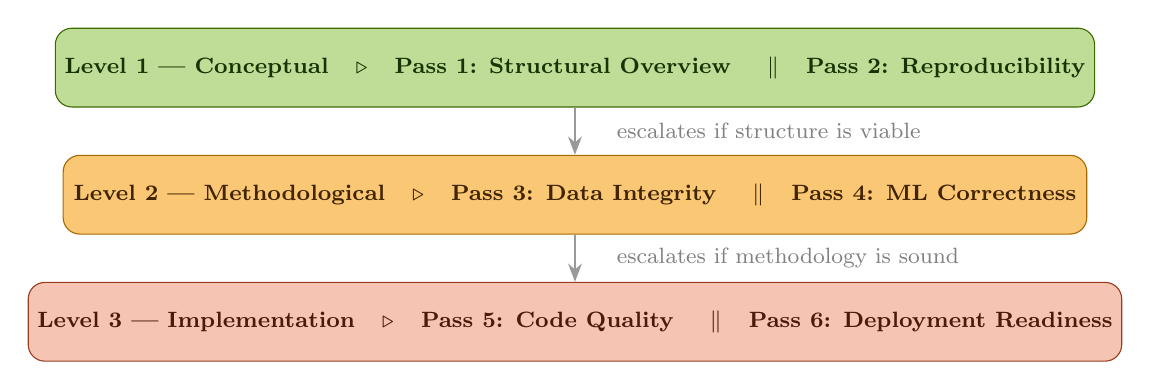
\begin{tikzpicture}[
    level/.style={
      rectangle, rounded corners=6pt, align=center,
      draw=black!60, font=\footnotesize\bfseries,
      minimum width=130mm, minimum height=10mm
    },
    lbl/.style={font=\footnotesize, text=black!50}
    ]

    \node[level, fill=greenFill, draw=greenStroke, text=greenTxt] (L1)
      {Level 1 — Conceptual\quad $\triangleright$\quad
       Pass 1: Structural Overview \quad$\|$\quad Pass 2: Reproducibility};

    \node[level, fill=amberFill, draw=amberStroke, text=amberTxt,
          below=6mm of L1] (L2)
      {Level 2 — Methodological\quad $\triangleright$\quad
       Pass 3: Data Integrity \quad$\|$\quad Pass 4: ML Correctness};

    \node[level, fill=coralFill, draw=coralStroke, text=coralTxt,
          below=6mm of L2] (L3)
      {Level 3 — Implementation\quad $\triangleright$\quad
       Pass 5: Code Quality \quad$\|$\quad Pass 6: Deployment Readiness};

    \draw[->, >=Stealth, line width=0.8pt, draw=black!40]
      (L1.south) -- node[lbl, right=4mm]{escalates if structure is viable}
      (L2.north);
    \draw[->, >=Stealth, line width=0.8pt, draw=black!40]
      (L2.south) -- node[lbl, right=4mm]{escalates if methodology is sound}
      (L3.north);

  \end{tikzpicture}
  \caption{Three-level audit hierarchy. Each level gates the next:
           Level~1 must confirm structural coherence before Level~2
           inspects methodology; Level~2 must confirm methodological
           soundness before Level~3 inspects code quality.}
  \label{fig:audit-levels}
\end{figure}

% ============================================================
\section{Prompt Engineering Evolution}
\label{sec:prompt-evolution}
% ============================================================

The prompt design for notebook auditing evolved through three iterations
(called ``Laps''), each increasing in specificity, output-structure demands,
and the number of distinct audit checks.

\subsection{Lap 1 — Coarse Evaluation}

A coarse, two-phase prompt that asks the model to produce documentation
(overall purpose, block descriptions, pseudocode, pipeline summary) and then
a critical audit (cross-block consistency, redundancy, contradictory logic,
missing error handling). The output is free-form text with minimal structure.

\subsection{Lap 2 — Refined Evaluation}

Introduces explicit formatting requirements: numbered blocks consolidated by
type (Environment Setup, then one per computational cell), mandatory metadata
per block (Logic Flow, Data Transformations, Model/Algorithm Operations, Key
Variables, Side Effects), and a cross-block code quality audit with bullet
categories (Coherence, Redundancy, Contradiction). Still free-form, but
machine-parseable.

\subsection{Lap 3 — Structured Evaluation (Three-Level Prompts)}

The current state: each of the three audit levels (Conceptual, Methodological,
Implementation) has its own dedicated prompt template. These templates are
self-contained, with explicit step-by-step instructions, output-format
constraints, and explicit \emph{scope boundaries} that forbid the model from
drifting into other audit levels' territory.

This is the prompt form used in the cross-LLM comparison methodology.

% ============================================================
\section{Sensor Prompt Methodology}
% ============================================================

The final iteration of the prompt strategy treats each LLM as an
\textbf{interchangeable sensor}. A single, fixed prompt — the ``sensor prompt''
— is sent to every model under test, along with the same notebook content. The
prompt contains strict constraints:

\begin{itemize}
  \item No scoring or severity labels (the sensor only extracts evidence).
  \item No aggregating multiple issues into one observation.
  \item Return only JSON matching the \texttt{SensorOutput} schema.
  \item Refuse a monolithic audit (return a \texttt{chunking-required} flag)
        if the notebook exceeds context limits.
\end{itemize}

\subsection{SensorOutput JSON Schema}

The single output shape every model must produce:

\begin{description}[leftmargin=*]
  \item[\texttt{overall\_purpose}] (string) 2--3 sentence summary of the
        notebook's goal.

  \item[\texttt{pipeline\_summary}] (string) 3--5 sentence summary of block
        dependencies and data flow.

  \item[\texttt{observations}] (array) One entry per (criterion, cell) pair.
        Each entry contains:
        \begin{itemize}
          \item \texttt{criterion\_id} — e.g., \texttt{"1.4"}, \texttt{"2.1"}
          \item \texttt{cell\_id} — stable cell identifier
          \item \texttt{applicability} — \texttt{IN\_SCOPE} or \texttt{NOT-APPLICABLE}
          \item \texttt{observation} — factual statement, no judgement words
          \item \texttt{code\_snippet} — exact snippet supporting the claim
          \item \texttt{line\_range} — e.g., \texttt{"C005:10-15"}
        \end{itemize}

  \item[\texttt{complex\_functions}] (array) Non-trivial functions translated
        to pseudocode. Each entry: \texttt{cell\_id}, \texttt{function\_name},
        \texttt{pseudocode}.

  \item[\texttt{cross\_reference\_discrepancies}] (array) Mismatches between
        the documented pipeline summary and the actual code.
\end{description}

\subsection{Audit Criteria}

The sensor prompt scans two fixed criteria groups:

\begin{table}[ht]
  \centering
  \caption{Audit criteria applied by the sensor prompt.}
  \renewcommand{\arraystretch}{1.2}
  \begin{tabular}{c l p{0.55\textwidth}}
    \toprule
    \textbf{ID} & \textbf{Criterion} & \textbf{What it checks} \\
    \midrule
    1.1 & Workflow Order & Whether cells follow a logical top-to-bottom
         progression matching the section structure. \\
    1.2 & Execution Order & Strictly linear execution; flag cells that depend
         on later cells. \\
    1.3 & Code Readability & Naming clarity, logical grouping, absence of
         monolithic cells. \\
    1.4 & Documentation & Markdown cells explaining intent and expected output
         for every code cell. \\
    \addlinespace
    2.1 & Environment Variables & Hardcoded paths, credentials, or
         environment-specific assumptions. \\
    2.2 & Reliable Data Handling & Data validation at ingestion, consistent
         split handling, leakage avoidance. \\
    2.3 & Atomic/Reusable Cells & Cell independence, explicit variable passing,
         no hidden state. \\
    2.4 & Reproducibility Controls & Random seeds set globally and consistently
         before any stochastic operation. \\
    2.5 & Caching/Fast Reruns & Mechanisms to avoid redundant computation on
         re-execution. \\
    \bottomrule
  \end{tabular}
  \label{tab:criteria}
\end{table}

% ============================================================
\section{LLMs Under Test}
% ============================================================

\subsection{Model Classification}

Models are classified into two types in the experiment configuration:

\begin{description}
  \item[\texttt{API}] Remote, cloud-hosted models accessed through a
        provider's HTTP endpoint (e.g., GPT-4, Claude). The app sends the
        prompt via a provider abstraction layer.

  \item[\texttt{Local}] Self-hosted models running on the user's hardware
        through the in-process llama.cpp server. The same OpenAI-compatible
        \texttt{/v1/chat/completions} interface is used regardless of
        whether the model is local or remote.
\end{description}

\subsection{Experiment Configuration}

The extended \texttt{input-experiment.json} template ties together the prompt,
the notebook, and the list of target models:

\begin{lstlisting}[style=json]
{
  "timestamp": "2026-07-10T20:00:00Z",
  "prompt": "You are a factual evidence-extraction sensor...",
  "notebookPath": "notebooks/example.ipynb",
  "models": [
    { "name": "gpt-4",       "type": "API"   },
    { "name": "claude-sonnet-5", "type": "API"   },
    { "name": "llama-3-8b",  "type": "Local", "quantization": "q4_0" }
  ]
}
\end{lstlisting}

\subsection{Output Collection}

The corresponding \texttt{output-experiment.json} captures each model's
response as a parsed \texttt{SensorOutput} object, together with timing
data:

\begin{lstlisting}[style=json]
{
  "timestamp": "2026-07-10T20:00:00Z",
  "outputs": [
    {
      "model": "gpt-4",
      "type": "API",
      "response": { "overall_purpose": "...", "observations": [...] },
      "delayResponse": "2026-07-10T20:00:04Z"
    }
  ]
}
\end{lstlisting}

% ── LLM Execution Flow Diagram ───────────────────────────────
\begin{figure}[ht]
  \centering
  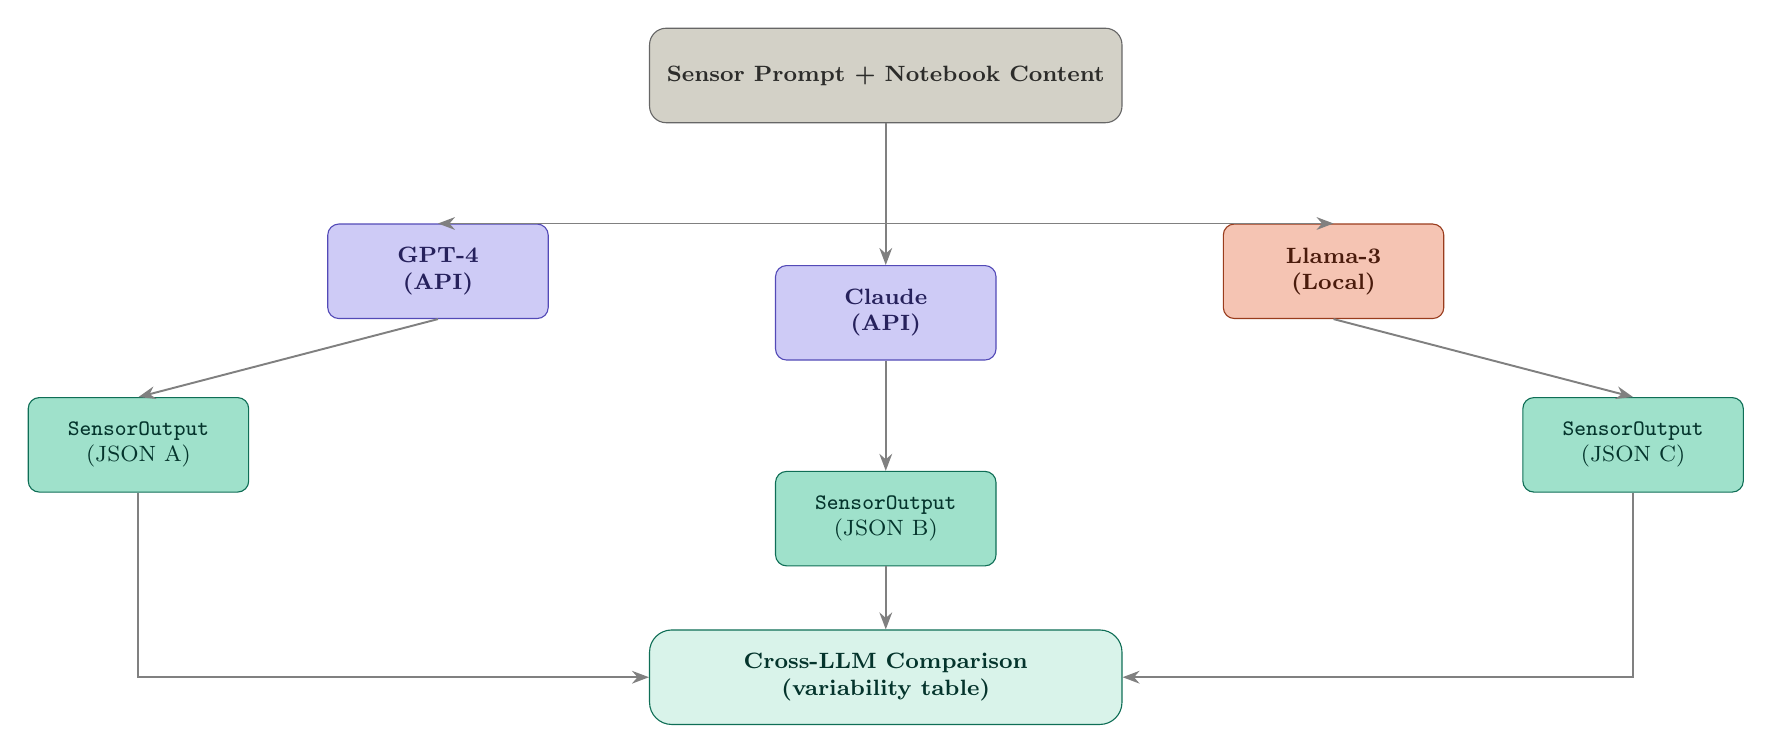
\begin{tikzpicture}[
    src/.style={
      rectangle, rounded corners=6pt, minimum width=60mm, minimum height=12mm,
      draw=black!60, fill=grayFill, text=grayTxt, align=center,
      font=\footnotesize\bfseries
    },
    api/.style={
      rectangle, rounded corners=4pt, minimum width=28mm, minimum height=12mm,
      draw=purpleStroke, fill=purpleFill, text=purpleTxt, align=center,
      font=\footnotesize\bfseries
    },
    loc/.style={
      rectangle, rounded corners=4pt, minimum width=28mm, minimum height=12mm,
      draw=coralStroke, fill=coralFill, text=coralTxt, align=center,
      font=\footnotesize\bfseries
    },
    outn/.style={
      rectangle, rounded corners=4pt, minimum width=28mm, minimum height=12mm,
      draw=tealStroke, fill=tealFill, text=tealTxt, align=center,
      font=\footnotesize
    },
    arr1/.style={->, >=Stealth, line width=0.7pt, draw=black!50},
    ]

    \node[src] (prompt) at (0,0)
      {Sensor Prompt + Notebook Content};

    \node[api, below left=18mm of prompt] (gpt)
      {GPT-4\\(API)};
    \node[api, below=18mm of prompt] (claude)
      {Claude\\(API)};
    \node[loc, below right=18mm of prompt] (llama)
      {Llama-3\\(Local)};

    \draw[arr1] (prompt.south) |- (gpt.north);
    \draw[arr1] (prompt.south) -- (claude.north);
    \draw[arr1] (prompt.south) |- (llama.north);

    \node[outn, below left=14mm of gpt] (outA)
      {\texttt{SensorOutput}\\(JSON A)};
    \node[outn, below=14mm of claude] (outB)
      {\texttt{SensorOutput}\\(JSON B)};
    \node[outn, below right=14mm of llama] (outC)
      {\texttt{SensorOutput}\\(JSON C)};

    \draw[arr1] (gpt.south) -- (outA.north);
    \draw[arr1] (claude.south) -- (outB.north);
    \draw[arr1] (llama.south) -- (outC.north);

    \node[rectangle, rounded corners=8pt, draw=tealStroke, fill=tealFill!40,
          text=tealTxt, align=center, minimum width=60mm, minimum height=12mm,
          font=\footnotesize\bfseries,
          below=8mm of outB] (comp)
      {Cross-LLM Comparison\\(variability table)};

    \draw[arr1] (outA.south) |- (comp.west);
    \draw[arr1] (outB.south) -- (comp.north);
    \draw[arr1] (outC.south) |- (comp.east);

  \end{tikzpicture}
  \caption{Execution flow: the same structured prompt and notebook are
           dispatched to each LLM; each returns a \texttt{SensorOutput}
           JSON object; all outputs are then compared in a unified
           variability table.}
  \label{fig:exec-flow}
\end{figure}

% ============================================================
\section{Cross-LLM Comparison}
% ============================================================

Because every model returns the same \texttt{SensorOutput} schema, outputs
from N models produce N structurally identical JSON files that can be
compared field-by-field. This is the core of the variability analysis.

\subsection{Comparison Table}

The comparison pivots the \texttt{observations} arrays from all models into
one table, keyed by \texttt{criterion\_id + cell\_id}, with one column per LLM:

\begin{table}[ht]
  \centering
  \caption{Example comparison table. A blank cell means the model did not emit
           an observation for that criterion--cell pair — itself a meaningful
           signal.}
  \renewcommand{\arraystretch}{1.4}
  \footnotesize
  \begin{tabularx}{\textwidth}{c c Y Y Y c}
    \toprule
    \textbf{Criterion} & \textbf{Cell} & \textbf{GPT-4} & \textbf{Claude} & \textbf{Llama-3} & \textbf{Variability} \\
    \midrule
    2.4 & C008
      & Seeds set for random, numpy, torch
      & Seeds set for random, numpy, torch
      & \textit{(absent)}
      & \textcolor{amberTxt}{partial} (2/3) \\
    \addlinespace
    2.1 & C005
      & DATA\_URL and RNG\_SEED hardcoded
      & Only RNG\_SEED flagged; DATA\_URL missed
      & Config values hardcoded
      & \textcolor{coralTxt}{divergent} \\
    \addlinespace
    1.1 & —
      & NOT-APPLICABLE
      & IN\_SCOPE
      & IN\_SCOPE
      & \textcolor{coralTxt}{applicability disagreement} \\
    \addlinespace
    1.3 & C003
      & Clear, well-named variables
      & Clear, well-named variables
      & Clear, well-named variables
      & \textcolor{greenTxt}{consistent} \\
    \bottomrule
  \end{tabularx}
  \label{tab:comparison}
\end{table}

\subsection{Variability Types}

Each comparison row is classified by the nature of disagreement:

\begin{description}[leftmargin=*]
  \item[\texttt{consistent}] All models agree in both coverage and content.
  \item[\texttt{missing-in-one}] One or more models skipped a cell/criterion
        the others covered.
  \item[\texttt{applicability-disagreement}] Models disagree on whether a
        criterion is \texttt{IN\_SCOPE} vs \texttt{NOT-APPLICABLE} for a cell.
  \item[\texttt{text-divergence}] All models reported something, but the
        factual content differs materially (different snippet, different scope).
\end{description}

\subsection{Variability Score}

A simple scalar metric per row and per notebook:

\[
\text{variabilityScore}_{\text{row}} = \frac{\text{number of models disagreeing with the majority}}{N_{\text{models}}}
\]

Aggregated across all rows, this gives a single ``how much do these models
agree'' number per notebook, useful for deciding whether a single model's audit
alone is trustworthy enough to skip cross-checking.

\subsection{\texttt{comparison-experiment.json} Artifact}

This structured artifact stores the full comparison for reproducibility:

\begin{lstlisting}[style=json]
{
  "timestamp": "2026-07-10T20:05:00Z",
  "notebookPath": "notebooks/example.ipynb",
  "models": ["gpt-4", "claude-sonnet-5", "llama-3-8b"],
  "comparisonRows": [
    {
      "criterion_id": "2.4",
      "cell_id": "C008",
      "byModel": {
        "gpt-4":    { "applicability": "IN_SCOPE", "observation": "..." },
        "claude":   { "applicability": "IN_SCOPE", "observation": "..." },
        "llama-3":  null
      },
      "variabilityScore": 0.33,
      "variabilityType": "missing-in-one"
    }
  ],
  "crossReferenceDiscrepancyDiff": {
    "onlyIn": {
      "gpt-4": [],
      "claude": ["pipeline_summary claims caching; C024 shows none"],
      "llama-3": []
    }
  }
}
\end{lstlisting}

% ============================================================
\section{Method Summary}
% ============================================================

The complete methodology for testing prompts and comparing LLMs as notebook
auditors consists of the following pipeline:

\begin{enumerate}[leftmargin=*]
  \item \textbf{Set up the execution environment.} Use the test-prompts-app
        to detect hardware, download GGUF models for local inference, and
        configure API credentials for remote models.

  \item \textbf{Define the experiment.} Populate
        \texttt{input-experiment.json} with the sensor prompt (or a
        level-specific audit prompt), the path to the target notebook,
        and the list of models under test.

  \item \textbf{Dispatch to all models.} The app sends the same prompt +
        notebook to every model. API models are called in parallel; local
        models share the server slot and are dispatched sequentially.

  \item \textbf{Collect structured outputs.} Each response is parsed and
        validated against the \texttt{SensorOutput} schema. Raw responses
        are preserved for traceability.

  \item \textbf{Compute the comparison.} Pivot the \texttt{observations}
        arrays into a unified table keyed by \texttt{criterion\_id +
        cell\_id}, with one column per model. Classify each row by
        variability type and compute a variability score.

  \item \textbf{Analyse variability.} Review rows flagged as
        \texttt{divergent}, \texttt{missing-in-one}, or
        \texttt{applicability-disagreement} — these are where a manual
        reviewer's attention is most valuable. Consistent rows may be
        accepted with lower scrutiny.

  \item \textbf{Store the comparison artifact.} Write
        \texttt{comparison-experiment.json} to disk for reproducibility
        and to enable comparison across notebooks and prompt versions.
\end{enumerate}

% ============================================================
\section{Project Structure (Relevant Components)}
% ============================================================

\begin{lstlisting}[style=json, basicstyle=\small\ttfamily]
test/prompts/
  app/
    api/
      local.py     -- hardware detection, HF browser, GGUF download,
                     AsyncLlamaServer (in-process inference server)
      utils.py     -- provider abstraction (dispatches prompt to
                     both API and Local models)
      compare.py   -- builds comparison rows / variability metrics
                     from a set of SensorOutput JSON files
    UI/
      app.py       -- Hardware / Models / Server / Settings / Compare tabs
  templates/
    input-experiment.json       -- prompt + notebook + model list
    output-experiment.json      -- per-model SensorOutput responses
    comparison-experiment.json  -- per-criterion/cell diff across models
  context/
    initial-idea.md    -- original multi-LLM comparison concept
    better-idea.md     -- refined sensor-prompt and cross-LLM design
    proposal/
      prompt-testing-methodology.tex  -- this document
  docs/                -- Sphinx autodoc for the app codebase
\end{lstlisting}

\vfill

\begin{center}
\rule{0.5\textwidth}{0.3pt}\\[6pt]
\small\textit{End of document.}
\end{center}

\end{document}
